
%-=============================================
\chapter{Metodología de la investigación}
%==============================================
%-------------------------------
\section{Diseño Metodológico}
%------------------------------
Hemos construido un sistema de reconocimiento de placas vehiculares, haciendo uso de redes neuronales convolucionales. El sistema fue creado realizando cambios en los parámetros de una RNC y, en cada cambio, ensayos de entrenamiento para observar el rendimiento; y así escoger la arquitectura que dio los mejores resultados. Por tal motivo, hemos considerado que se trata de una investigación de tipo experimental. 

El objetivo es diseñar un sistema experto que permita reconocer en una imagen de una placa colombiana, los 6 caracteres que ésta contiene. Con el fin de lograr este objetivo y responder cada una de las preguntas de investigación, hemos realizado el siguiente procedimiento:

\begin{itemize}

\item[i.] Estudio de todo lo relacionado con las RNC: Conocer su historia; los campos de aplicación; las diferentes arquitecturas y su estructura interna; los requerimientos de la base de datos para su entrenamiento; las herramientas computacionales para su implementación; las formas de medir su rendimiento; entre otros (ver sección \ref{marcoteorico}). Esta etapa nos motivó inicialmente a construir desde cero nuestra propia RNC; y luego, a usar la técnica de detección de objetos. 
    
\item[ii.] Construcción de una base de datos a partir de imágenes segmentadas de caracteres de placas colombianas. Tal base de datos la hemos llamado \textit{CharsPlateCol}. 
    
\item[iii.] Construcción de una RNC desde cero para ser entrenada con la base de datos construida \textit{CharsPlateCol}.
    
\item[iv.] Construcción de una base de datos de caracteres similares a los caracteres que se presentan en placas colombianas a partir de depuración de la base de datos pública \textit{Chars74k}. Tal base de datos la hemos llamado \textit{Chars34k}. 
    
\item[v.] Entrenamiento de la RNC construida desde cero, usando la base de datos \textit{CharsPlateCol} construida inicialmente, más la base de datos \textit{Chars34k}.
    
\item[vi.] Construcción de una base de datos usando cuadros delimitadores (Bonding Boxing) en imagenes de placas colombianas. Tal base de datos la hemos llamado \textit{CharsBoxPlateCol}.
 
 \item[vii.] Implementación de transferencia de aprendizaje para el entrenamiento de una Faster R-CNN usando la base de datos \textit{CharsBoxPlateCol} .
    \end{itemize}
%__________________________
%    \item Estudio del procesamiento de imágenes con la librería \textit{OpenCv} (ver sección  \ref{opencv}).

 %   \item Construcción de un código en \textit{Python} usando librería de \textit{OpenCv}, para realizar la segmentación de la placa y sus 6 caracteres. Estas imágenes  la entrada de nuestra RNC entrenada previamente.
    
  %  \item Construir una base de datos con imágenes de 40 x 80 píxeles con alta variabilidad en cada una de las 36 clases, obtenidas inicialmente de placas colombianas reales, luego realizamos el entrenamiento de la RCN con esta data.
    
    
 %   \item A nuestro dataset de placas colombianas construido anteriormente, le anexamos imágenes a cada una de las 36 clases de la data publica Chars74k, para explorar si se mejora el rendimiento de la Red neuronal convolucional.
    
  %  \item Construir un dataset para el entrenamiento de una Faster R-CNN.
    
  %  \item Entrenar una Faster R-CNN con nuestra data y por medio de la inferencia, que es el uso de redes pre-entrenadas
   
 %   \item Calcular todas las métricas de rendimiento de nuestra red neuronal y de la Faster R-CNN, para así responder las preguntas de investigación. 

%------------------------------------
\section{Datos y técnicas de recolección}
%--------------------------------------
La eficacia de un sistema de clasificación de imágenes basado en una red neuronal convolucional depende tanto de la arquitectura y ajustes de la red, como del conjunto de datos empleado para su entrenamiento. Este último debe ser suficientemente amplio y representativo del problema que se quiere resolver.

Nuestro objetivo es diseñar un sistema de visión artificial para el reconocimiento de placas de automóviles colombianos a partir de la imagen de la parte frontal del vehículo, de tal forma que se pudiesen distinguir, por un ojo humano normal, su placa; aunque no necesariamente todos los 6 caracteres que la componen. Este sistema puede ser implementado para el control de acceso a vehículos, en lugares tales como  parqueaderos.

En nuestro caso, para tener una base de datos adecuada a la aplicación que se quiere implementar, inicialmente hemos usado imágenes de vehículos tomadas por cámaras instaladas en parqueaderos de centros comerciales en Colombia. Estás imágenes fueros tomadas en condiciones ambientales reales. Esta base de datos la hemos llamado \textit{CharsPlateCol} y garantiza en cierta medida la variabilidad en condiciones ambientales que se exige en el entrenamiento de una RNC. Luego, para ampliar la base de datos construida, hemos escogido caracteres de la base de datos pública \textit{Chars74k}. Esta base de datos la hemos llamado \textit{Chars34k}. Finalmente, hemos construido una base de datos llamada \textit{CharsBoxPlateCol}. Esta base de datos fue especialmente construida para aplicar la técnica de detección de objetos; en este caso, los objetos a detectar son los caracteres de las placas.  
A continuación describiremos las bases de datos construidas:

%En primera instancia analizaremos la construcción de la data de caracteres segmentados y luego la data chars74K, debemos tener presente que este conjunto de datos está formado por 36 clases, que representa 10 dígitos y 26 letras que son las usadas en el formato de 3 letras y 3 números en las placas colombianas. 


\subsection{Base de datos \textit{CharsPlateCol}} \label{CharsPlateCol2.5k}

Esta base de datos de imágenes de caracteres de placas colombianas, ha sido construida a partir de imágenes capturadas con una cámara instalada en un parqueadero tal como se muestra en la figura \ref{fig:imagen completa}. 

\begin{figure}[H]
\centering
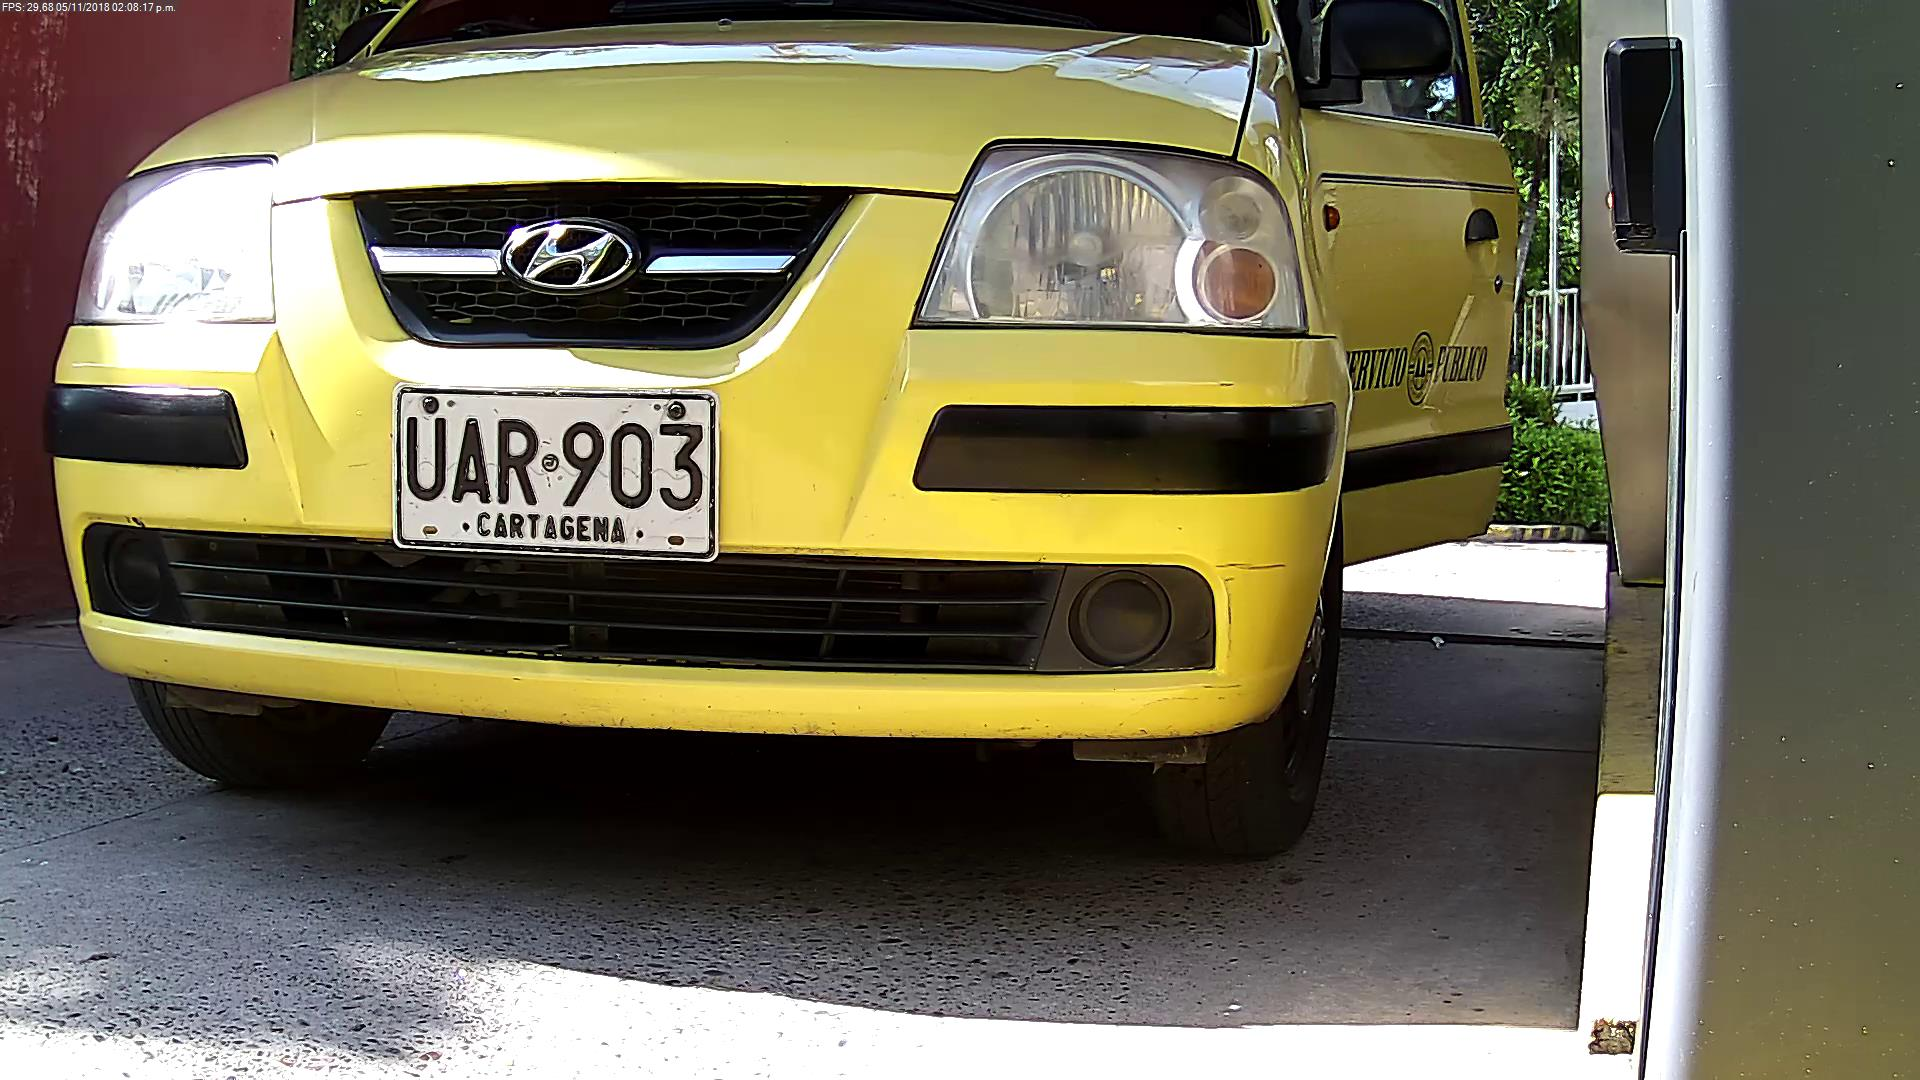
\includegraphics[width=0.7\linewidth]{imagenes/MODELO_4/segmentacion/carro4.jpg} 
\caption{ Cargamos Imagen}
\label{fig:imagen completa}
\end{figure}

La extracción de los caracteres se realizó con la librería OpenCV para el tratamiento de imágenes (ver sección \ref{opencv}). Seguidamente se explicará el proceso realizado, tomando como ejemplo la imagen del automovil mostrado en la figura \ref{fig:imagen completa}:    

 \begin{enumerate}
     \item  Se recorta la imagen para disminuir la región donde se encuentra la placa y facilitar el proceso de extracción. El resultado se muestra en la figura(\ref{fig:recorter}).
     
    \begin{figure}[H]
    \centering
    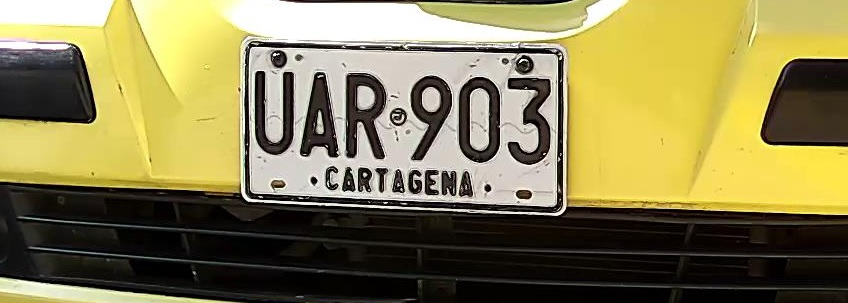
\includegraphics[width=0.5 \linewidth]{imagenes/MODELO_4/segmentacion/recorte.jpg} 
    \caption{ Recorte de la imagen}
    \label{fig:recorter}
    \end{figure}
     
     \item Se convierte a escala de grises. El resultado se muestra en la figura \ref{fig:Escala de grises}.
     
     \begin{figure}[H]
    \centering
    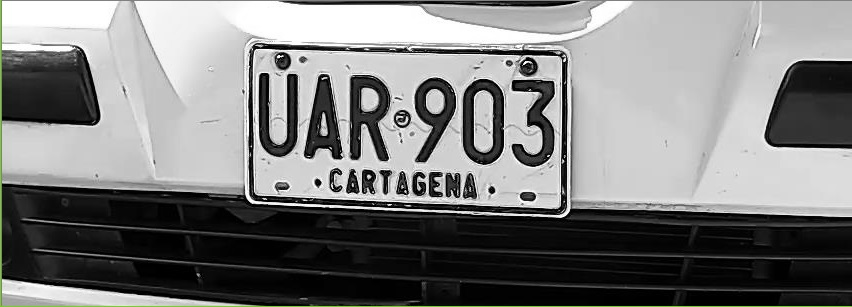
\includegraphics[width=0.5 \linewidth]{imagenes/MODELO_4/segmentacion/gris.jpg} 
    \caption{ Escala de grises}
    \label{fig:Escala de grises}
    \end{figure}
    
     \item Se convierte a una imagen a binaria (solamente ceros y unos). El resultado se observa en la figura \ref{fig:Convertimos la imagen a binaria}
     
     \begin{figure}[H]
    \centering
    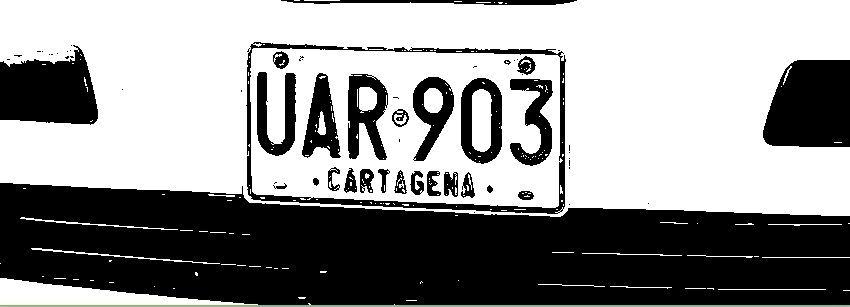
\includegraphics[width=0.5 \linewidth]{imagenes/MODELO_4/segmentacion/umbral.jpg} \caption{Convertimos la imagen a binaria}
    \label{fig:Convertimos la imagen a binaria}
    \end{figure}
     
     \item  se realiza un desenfoque Gaussiano para ampliar la frontera de los bordes. El resultado se aprecia en la figura \ref{fig:Desenfoque Gaussiano}.
     
     \begin{figure}[H]
    \centering
    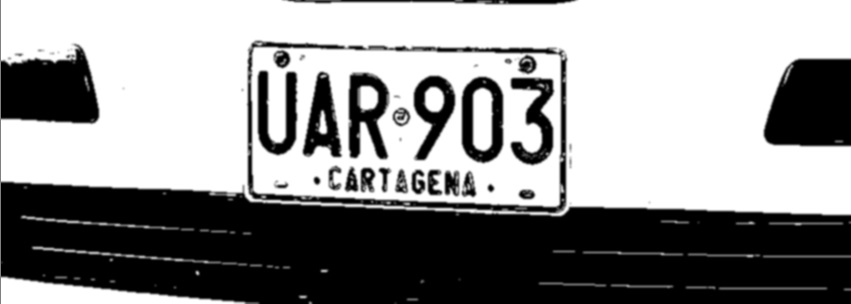
\includegraphics[width=0.5 \linewidth]{imagenes/MODELO_4/segmentacion/suavi.jpg} 
    \caption{Desenfoque Gaussiano}
    \label{fig:Desenfoque Gaussiano}
    \end{figure}
     
     \item Se resaltan los bordes con un filtro Canny. El resultado se puede ver en la figura \ref{fig:Bordes con Canny}.
     
     \begin{figure}[H]
    \centering
    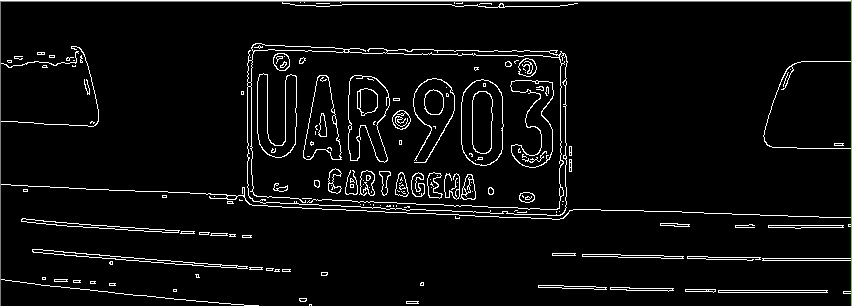
\includegraphics[width=0.5 \linewidth]{imagenes/MODELO_4/segmentacion/borde.jpg} 
    \caption{Bordes con Canny}
    \label{fig:Bordes con Canny}
    \end{figure}
    
     \item Se identifica la región de interés. El resultado se ve en la figura \ref{fig:Region ROI}, donde las lineas verdes son todos los contornos identificados y el cuadro  azul es la zona de interés (la placa).
     
     \begin{figure}[H]
    \centering
    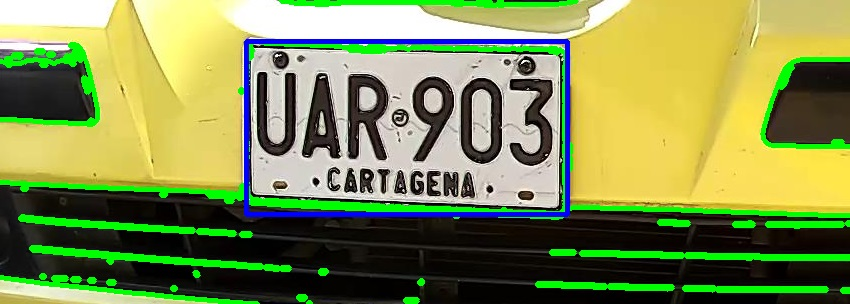
\includegraphics[width=0.5 \linewidth]{imagenes/MODELO_4/segmentacion/roi.jpg}
    \caption{Región de interés}
    \label{fig:Region ROI}
    \end{figure}

    
    \item Se recorta la región de interés. El resultado se observa en la figura \ref{fig:Extracción placa}.
     
     \begin{figure}[H]
    \centering
    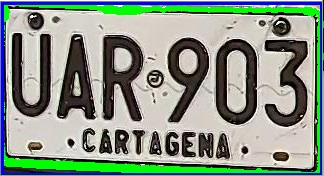
\includegraphics[width=0.5 \linewidth]{imagenes/MODELO_4/segmentacion/placa.jpg} 
    \caption{Extracción placa}
    \label{fig:Extracción placa}
    \end{figure}
     
     \item Finalmente de la placa segmentada se recortan los caracteres. El resulyado se puede observar en la figura \ref{fig:segmentación de caracteres}. Son estos caracteres los que hacen parte de la base de datos construida.

    \begin{figure}[H]
    \centering
    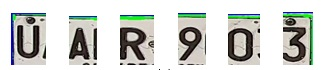
\includegraphics[width=0.6 \linewidth]{imagenes/MODELO_4/segmentacion/segmentacion_figura2.jpg} \caption{segmentación de caracteres}
    \label{fig:segmentación de caracteres}
    \end{figure}
     
 \end{enumerate}
 
 %     \begin{figure}[H]
  %  \centering
   % 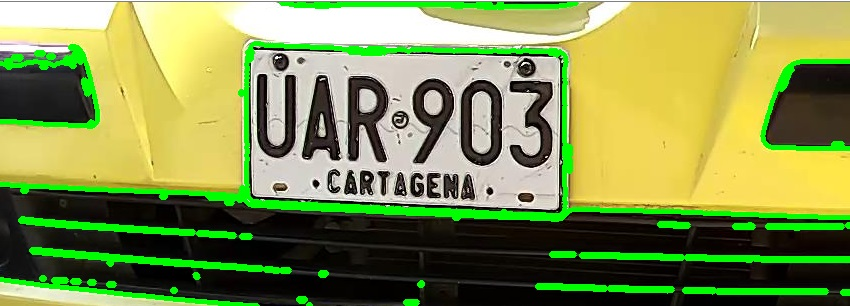
\includegraphics[width=0.5 \linewidth]{imagenes/MODELO_4/segmentacion/contor.jpg} 
    %\caption{Identificar y dibujar contornos}
    %\label{fig:Identificar y dibujar contornos}
    %\end{figure}


%\end{enumerate}


%La red neuronal convolucional que será entrenada con esta base de datos, tiene que clasificar los 6 caracteres de placas colombianas diseñadas con 3 letras y 3 números. Por tal motivo, hicimos el proceso descrito anteriormente con placas reales que se lograron segmentar. 

En total se segmentaron 432 placas. La figura \ref{fig:Muestra de placas segmentadas} es una muestra de las placas colombianas una vez segmentadas y que fueron usadas para obtener cada uno de los caracteres de la base de datos \textit{CharsPlateCol2.5k}

\begin{figure}[H]
  {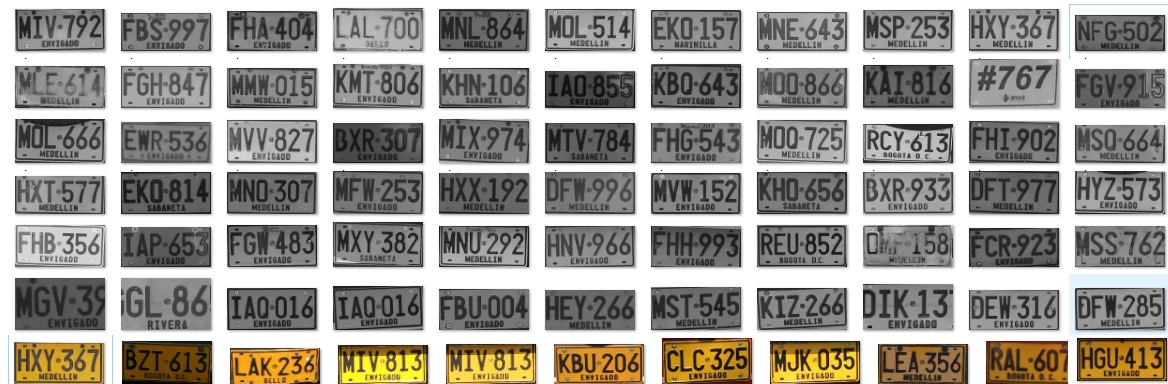
\includegraphics[width=1\linewidth]{imagenes/RESULTADOS/PLACAS_PA_SEGMENTAR.jpg}}
   \caption{Muestra de placas segmentadas}
    \label{fig:Muestra de placas segmentadas}  
\end{figure}

%Con las placas segmentadas, la siguiente etapa es el proceso de segmentación que se realizó inicialmente de forma manual. Luego, se diseñó un código para la segmentación automática de los 6 caracteres por placa, 

La base de datos \textit{CharsPlateCol2.5k} así construida, tiene un total de 2593 imágenes de caracteres (letras y números) con un tamaño de 40 x 80 píxeles con 3 canales. En la figura \ref{fig:Muestra caracter D base de datos} se puede observar una muestra de letras D pertenecientes a la base de datos construida.

\begin{figure}[H]
  {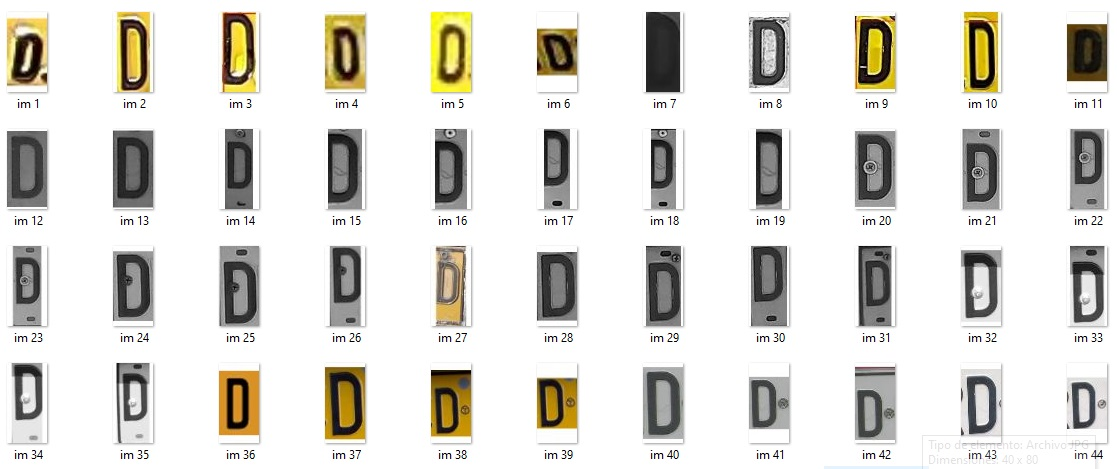
\includegraphics[width=1\linewidth]{imagenes/RESULTADOS/muestra_letra.jpg}}
   \caption{Muestra caracter D base de datos segmentadas \textit{CharsPlateCol}}
    \label{fig:Muestra caracter D base de datos}
\end{figure} 

En la base de datos se distinguen 36 clases: 10 números del 0 al 9 y 26 letras del alfabeto español. En el cuadro \ref{table:Caracteres por clase} se muestra la cantidad de imágenes que tenemos en cada clase y en la figura \ref{fig:frecuencia} un diagrama de frecuencias. 

\begin{table}[H]
\begin{center}
\resizebox{0.5\textwidth}{!}{
\begin{tabular}{||c|c|
|c|c||}
\hline
 Clase & Frecuencia & Clase & Frecuencia\\
\hline \hline
000 & 106 & letra I & 106\\\hline
001 & 55 & letra J & 60\\\hline
002 & 62 & \textcolor{red}{letra K} & \textcolor{red}{50}\\\hline
\textcolor{green}{003} & \textcolor{green}{111} & letra L & 54\\\hline
004 & 61 & letra M & 62\\\hline
005 & 62 & letra N & 94\\\hline
006 & 72 & letra O & 99\\\hline
\textcolor{red}{007}&\textcolor{red}{ 50} & letra P & 51\\\hline
008 & 56 & letra Q & 57\\\hline
009 & 52 & letra R & 70\\\hline
letra A & 59 & letra S & 101\\\hline
\textcolor{red}{letra B} & \textcolor{red}{50} & letra T & 54\\\hline
\textcolor{green}{letra C} & \textcolor{green}{120} & letra U & 112\\\hline
letra D & 89 & letra V & 54\\\hline
letra E & 55 & letra W & 54\\\hline
letra F & 51 & letra X & 105\\\hline
letra G & 62 & letra Y & 115\\\hline
letra H & 58 & letra Z & 63\\ \hline
\hline
Total imágenes & \multicolumn{3}{|c||}{2593}\\
\hline \hline
\end{tabular}
}
\caption{\label{table:Caracteres por clase}Cantidad de imágenes por clase en la base de datos \textit{CharsPlateCol}}
\end{center}
\end{table}

\begin{figure}[H]
\centering
  {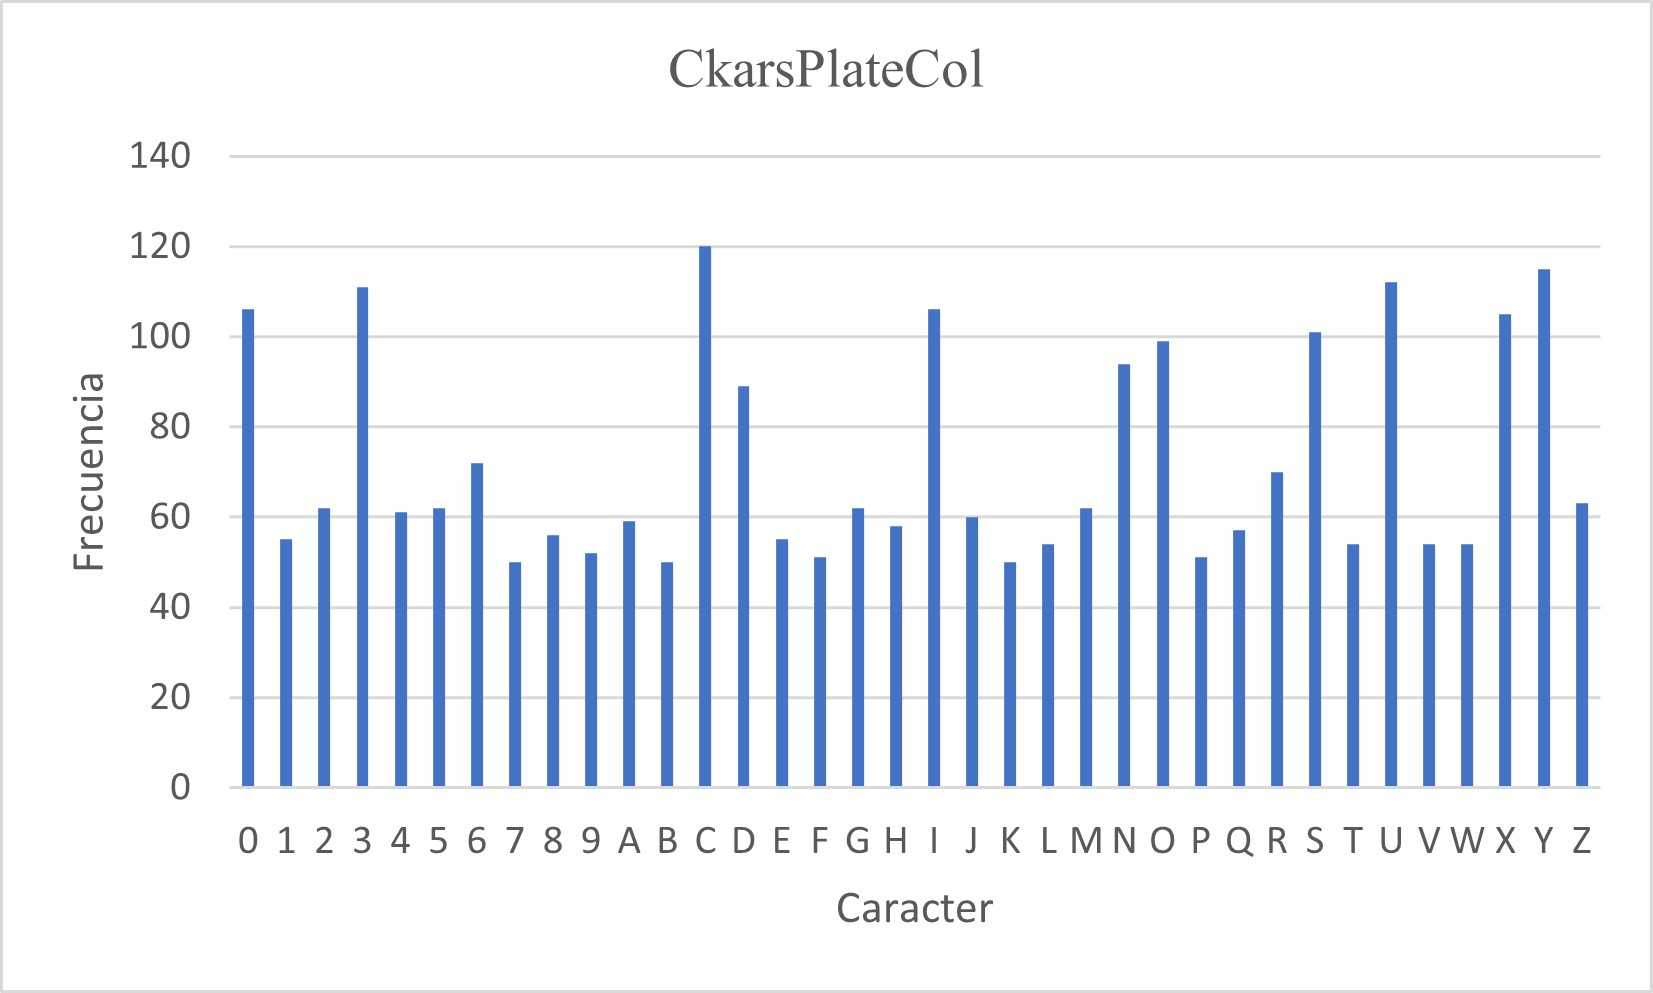
\includegraphics[width=0.8\linewidth]{imagenes/frecuenciaCaracter1.jpg}}
   \caption{Frecuencia de cada caracter en la base de datos \textit{CharsPlateCol}}
    \label{fig:frecuencia}
\end{figure} 

Se puede observar que la distribución de la cantidad de imágenes por cada carácter no es la misma, ya que en las 432 placas, no se encontraban la misma cantidad de caracteres. Lo que indica, que nuestra base de datos es heterogénea con relación al número imágenes por caracter. Esta heterogeneidad puede deberse a que las imágenes fueron tomadas en una misma ciudad y tienden a repetirse unos caracteres más que otros.  

%Con las 36 clases definidas, que representa cada uno de los caracteres, realizamos el conteo de los caracteres por clase, y encontramos que prevalecen las imágenes de la letra \textbf{C} con 120 de ellas y el número \textbf{3} con 111, debemos resaltar que tenemos caracteres con solo 50 imágenes, fue así, y logramos crear una data con un total de 2593 imágenes. 


\subsection{Base de datos \textit{Chars34k}} \label{Chars34k}

Como no se tenía una base de datos de diferentes ciudades colombianas para tener una base de datos un poco más homogénea, se decidió completarla con caracteres de la base de datos pública \textit{Chars74k} (ver sección \ref{Chars74k}). Este dataset cuenta con 74.000 imágenes de números y letras con mucha variabilidad y estilos. En la figura \ref{fig:Muestra de dataset chars74K} se observa una muestra de caracteres de tal base de datos. En este conjunto no todos los caracteres son similares a los usados en las placas colombianas, por ejemplo la base de datos tiene caracteres en minúsculas y las placas colombianas solamente usan caracteres en mayúsculas. Es así, que se hizo necesario realizar una depuración para escoger finalmente, un conjunto de aproximadamente 34 mil imágenes de caracteres (números y letras)  similares a los usados en las placas colombianas. Por tal razón, hemos llamado está base de datos \textit{Chars34k}.     
%-------------------------
%entrenar la red neuronal del sistema propuesto se ha elegido el conjunto de  datos \textit{Chars74k} (ver sección \ref{Chars74k}), Este dataset cuenta con más de 74.000 imágenes de números y letras, con mucha variabilidad, lo implica realizar necesariamente una depuración, para así escoger aquellas imágenes similares a los caracteres usados en placas Colombianas.

\begin{figure}[H]
\begin{center}
   {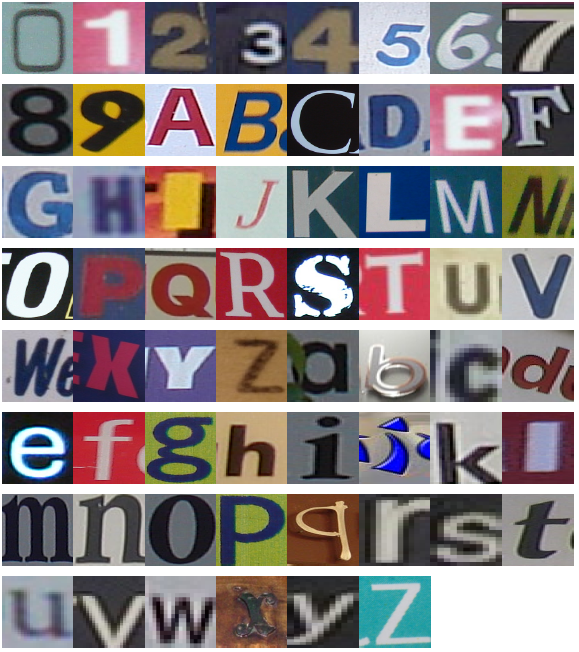
\includegraphics[width=.37\linewidth]{charks74.png}}
    \caption{Muestra de dataset chars74K}
    \label{fig:Muestra de dataset chars74K} 
\end{center}
\end{figure}

 %Esta depuración inicialmente fue solo de las letras minúsculas, puesto que las placas colombianas solo usan letras mayúsculas y dígitos, así que se revisamos más de 60 carpetas y se logró obtener 41772 archivos, distribuidos en 36 directorios, que representan 26 letras y 10 números.

%Se hizo este proceso de depuración en varias ocasiones, hasta obtener los caracteres semejantes a los usados en las placas colombianas.

\subsection{Base de datos conformada por \textit{Chars34k} y \textit{CharsPlateCol}} \label{Chars34k}

Para tener una base de datos mejor balanceada y representativa, se unieron las bases de datos \textit{CharsPlateCol2.5k} y \textit{Chars34k}. En la figura \ref{fig:Muestra de dataset chars34K} se puede observar una muestra con imágenes de la letra G tanto de placas colombianas como de la base de datos \textit{Chars34k}. 
%tomaron cerca de 1000 placas colombianas y se segmentaron sus caracteres con el objetivo de balancear la data a usar en el entrenamiento de la Red neuronal convolucional, con 37.398 imágenes de 40 x 80 píxeles distribuidas en 36 carpetas. La figura \ref{fig:Muestra de dataset chars34K} es la muestra de la letra G en la base de datos \textit{chars34K}, que incluye letras de placas colombianas y letras depuradas de la base de datos \textit{chars74K}.
\begin{figure}[H]
\begin{center}
   \subfigure[]{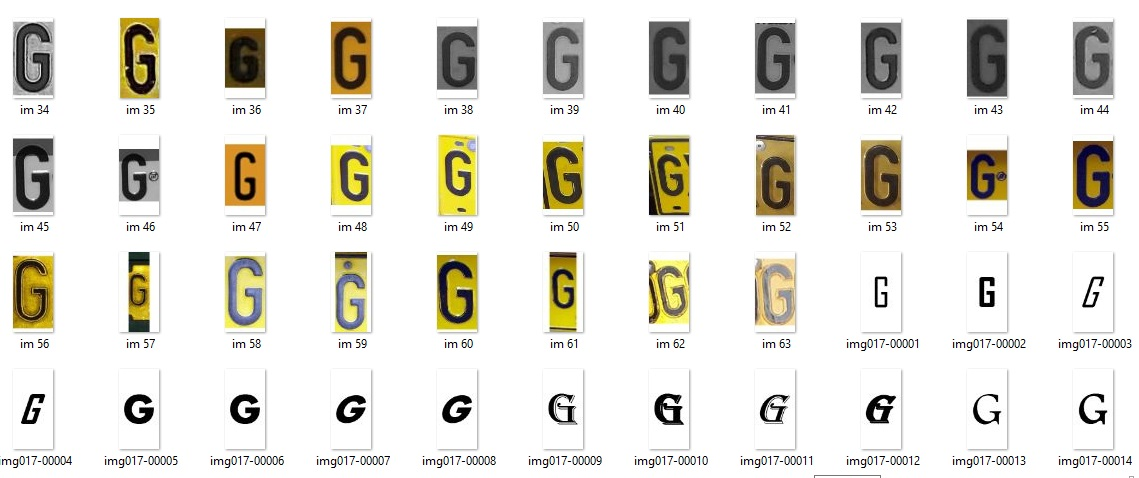
\includegraphics[width=.9\linewidth]{muestra_data.jpg}}
    \caption{Una muestra de imagenes de la letra G tanto en \textit{Chars34k} y \textit{CharsPlateCol}}
    \label{fig:Muestra de dataset chars34K} 
\end{center}
\end{figure}

En el cuadro \ref{table:Caracteres por clase} se muestra la cantidad de imágenes en cada clase y en la figura \ref{fig:frecuencia2} un diagrama de frecuencias. El conjunto total contiene 37.398 imágenes con tamaño de 40x80 píxeles. Se puede observar en el diagrama que se obtiene una base de datos mejor balanceada, salvo el número 8 que tiene menos frecuencia.

%Luego de la construcción de la data \textit{chars34K}, contabilizamos el número de caracteres por clase, y encontramos que prevalecen las imágenes de la letra \textbf{X} con 2065 de ellas y el número \textbf{3} con 1162

\begin{table}[H]
\begin{center}
\resizebox{0.5\textwidth}{!}{
\begin{tabular}{||c|c||c|c||}
\hline \hline
 Clase & Frecuencia & Clase & Frecuencia\\
\hline\hline
000  &  1134 & letra I  &  1118\\\hline
001  &  1035 & letra J  &  1035\\\hline
002  &  1018 & letra K & 997\\\hline
\textcolor{green}{003}  & \textcolor{green}{ 1162} & letra L & 949\\\hline
004 &  1026 & letra M  &  1012\\\hline
005 & 971 & letra N  &  1075\\\hline
006 & 993 & letra O  &  1105\\\hline
007  &  1018 & letra P  &  1002\\\hline
\textcolor{red}{008} & \textcolor{red}{86} & \textcolor{red}{letra Q} &\textcolor{red}{ 886}\\\hline
009 & 995 & letra R & 999\\\hline
letra A  &  1025 & letra S  &  1102\\\hline
letra B  &  1016 & letra T  &  1001\\\hline
letra C  &  1173 & letra V & 994\\\hline
letra D  &  1117 & letra U  &  1121\\\hline
letra E  &  1023 & letra W  &  1005\\\hline
letra F & 991 & \textcolor{green}{letra X} & \textcolor{green}{2065}\\\hline
letra G  &  1036 & letra Y  &  1104\\\hline
letra H & 986 & letra Z  &  1022\\
\hline \hline
Total imágenes & \multicolumn{3}{|c|}{37397} \\
\hline \hline
\end{tabular}
}
\caption{\label{table:imagenes por clase chars74k}Cantidad de imágenes por clase en la base de datos obtenida al unir \textit{Chars74k} con \textit{CharsPlateCol}}
\end{center}
\end{table}

\begin{figure}[H]
\centering
  {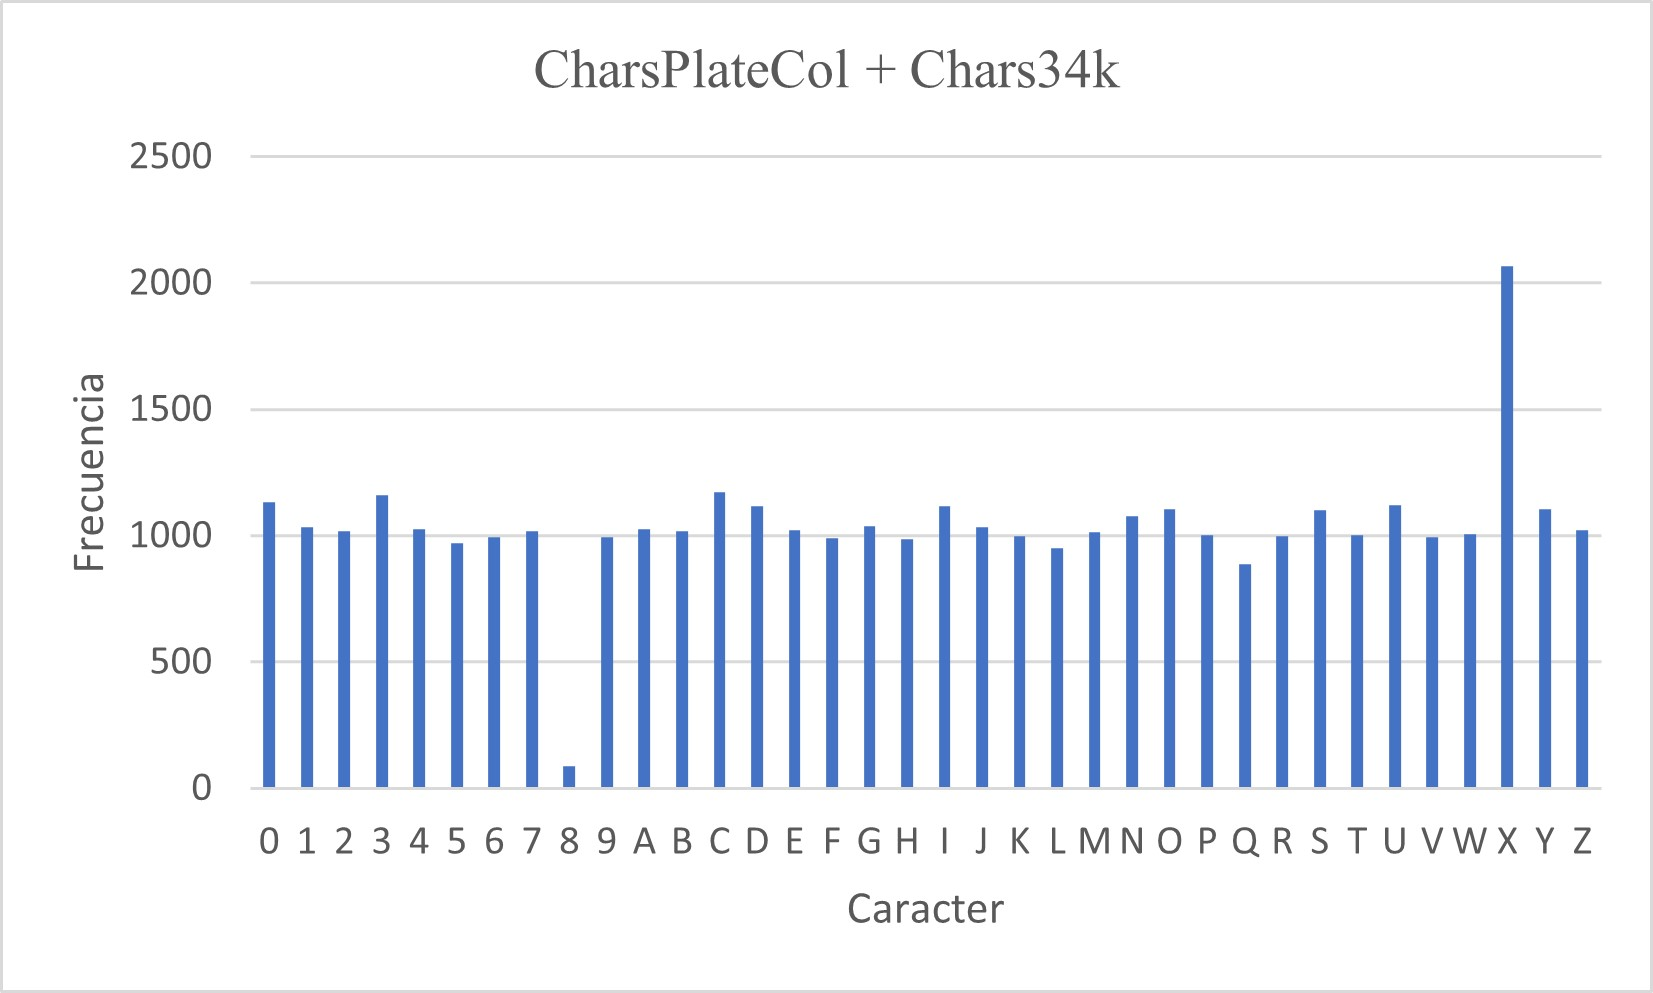
\includegraphics[width=0.8\linewidth]{imagenes/frecuenciaCaracter2.jpg}}
   \caption{Frecuencia de cada caracter en la base de datos resultante de unir \textit{Chars34k} con \textit{CharsPlateCol}}.
    \label{fig:frecuencia2}
\end{figure}

%-----------------------------------------------------
\subsection{Base de datos \textit{CharsBoxPlateCol}} \label{sec:basedatos3}
%----------------------------------------------------
Esta base de datos se ha construido para realizar transferencia de aprendizaje usando el modelo Faster R-CNN Inception v2 (COCO) de TensorFlow. Este modelo utiliza la técnica de detección de objetos (ver sección \ref{sec:deteccionobjetos}). La base de datos para el entrenamiento de este tipo de modelos debe incluir, además de la imagen de la placa, las coordenadas del rectángulo donde esta inscrito cada caracter a ser detectado. 
El proceso para obtener las coordenadas del objeto, en este caso de cada caracter, dentro de la imagen, se denomina Etiquetado (Labeling). Nosotros hemos realizado el proceso de etiquetado usando la aplicación \textbf{LabelImg}. Esta aplicación tiene una interfaz que permite al usuario delimitar con un rectángulo (Bonding box) cada uno de los caracteres dentro de la imagen y realizar el etiquetado con la clase correspondiente. La figura \ref{fig:etiquetas deteccion} muestra un ejemplo del funcionamiento de la interfaz. El usuario va colocando los rectángulos delimitadores sobre los caracteres B,X,U,3,0 y 4; en un submenú a la derecha  va escogiendo la etiqueta correspondiente a cada caracter dentro del rectángulo.   

\begin{figure}[H]
\centering
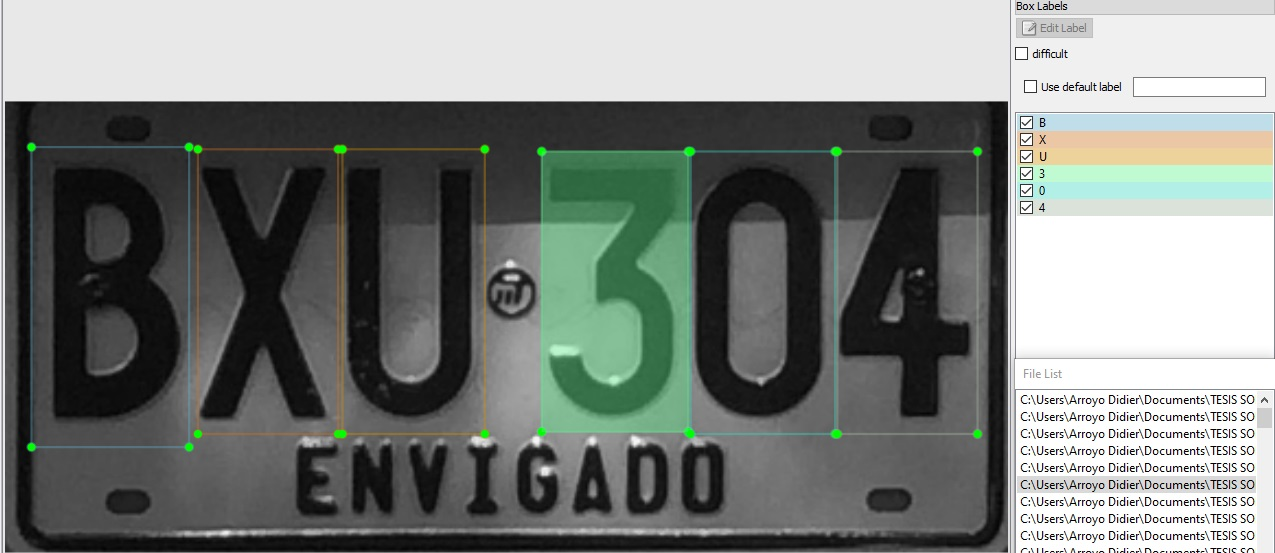
\includegraphics[width=0.5\textwidth]{imagenes/MODELO_5/ETIQUETA_MOD_IV.jpg} \caption{Aplicación LabelImg. Ejemplo de su interfaz de usuario para la obtención de las coordenadas del rectangulo delimitador}
\label{fig:etiquetas deteccion}
\end{figure}
 La aplicación genera un archivo en formato \textbf{Xml} con las coordenadas de cada uno de los rectangulos para cada clase (caracter) dentro de la imagen de la placa.  
 
\begin{figure}[H]
\centering
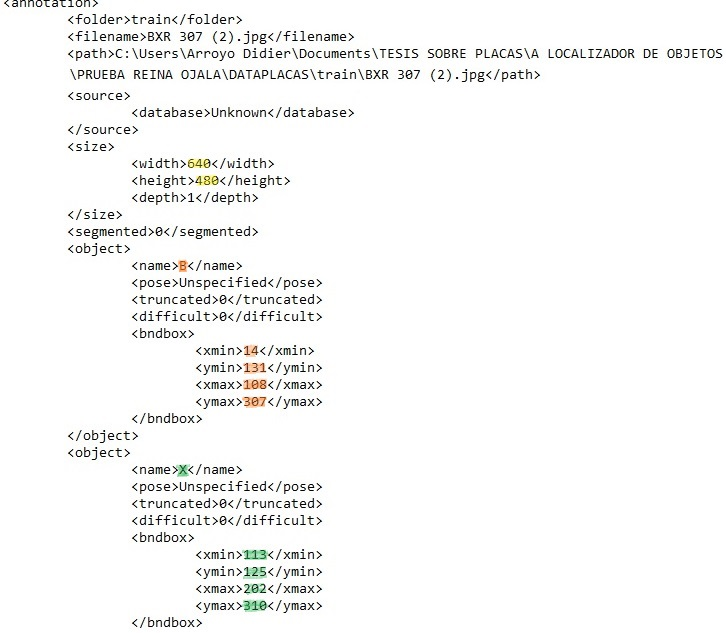
\includegraphics[width=0.7\linewidth]{imagenes/RESULTADOS/annonations.jpg} \caption{Archivo Xml generado por LabelIng para la placa en la Figura \ref{fig:etiquetas deteccion}.}
\label{fig:Ejemplo anotación Xml}
\end{figure}
 
 
 La Figura \ref{fig:Ejemplo anotación Xml} muestra una parte del contenido del archivo generado para el ejemplo considerado. Allí podemos ver (resaltados con colores) el tamaño de la placa y las coordenadas de las letras B y X.
Para nuestra base de datos se escogieron 177 placas, resultando en total 888 caracteres etiquetados. En la tabla \ref{table:frecuencia3} se muestra la cantidad de imágenes en cada clase y en la figura \ref{fig:frecuencia3} un diagrama de frecuencias. Se puede observar en el diagrama que se obtiene una base de datos muy desbalanceada.

\begin{table}[H]
\begin{center}
\resizebox{0.5\textwidth}{!}{
\begin{tabular}{||c|c||c|c||}
\hline \hline
 Clase & Frecuencia & Clase & Frecuencia\\
\hline\hline
000  &  36 & letra I  &  20\\\hline
001  &  27 & letra J  &  3\\\hline
002  &  39 & letra K & 28\\\hline
003  & 53 & letra L & 21\\\hline
004 &  47 & letra M  &  52\\\hline
005 & 53 & letra N  &  15\\\hline
006 & 55 & letra O  &  21\\\hline
007  &  41 & letra P  &  6\\\hline
008 & 28 & letra Q & 13\\ \hline
009 & 33 & letra R & 14\\\hline
letra A  &  18 & letra S  &  11\\\hline
letra B  &  19 & letra T  &  13\\\hline
letra C  &  3 & letra u & 12\\\hline
letra D  &  15 & letra v  &  21\\\hline
letra E  &  18 & letra W  &  16\\\hline
letra F & 47 & letra X & 21 \\\hline
letra G  &  16 & letra Y  &  9\\\hline
letra H & 39 & letra Z  &  5\\
\hline \hline
Total etiquetas & \multicolumn{3}{|c|}{888} \\
\hline \hline
\end{tabular}
}
\caption{\label{table:frecuencia3}Cantidad de etiquetas por clase en la base de datos\textit{CharsBoxPlateCol}}
\end{center}
\end{table}

\begin{figure}[H]
\centering
  {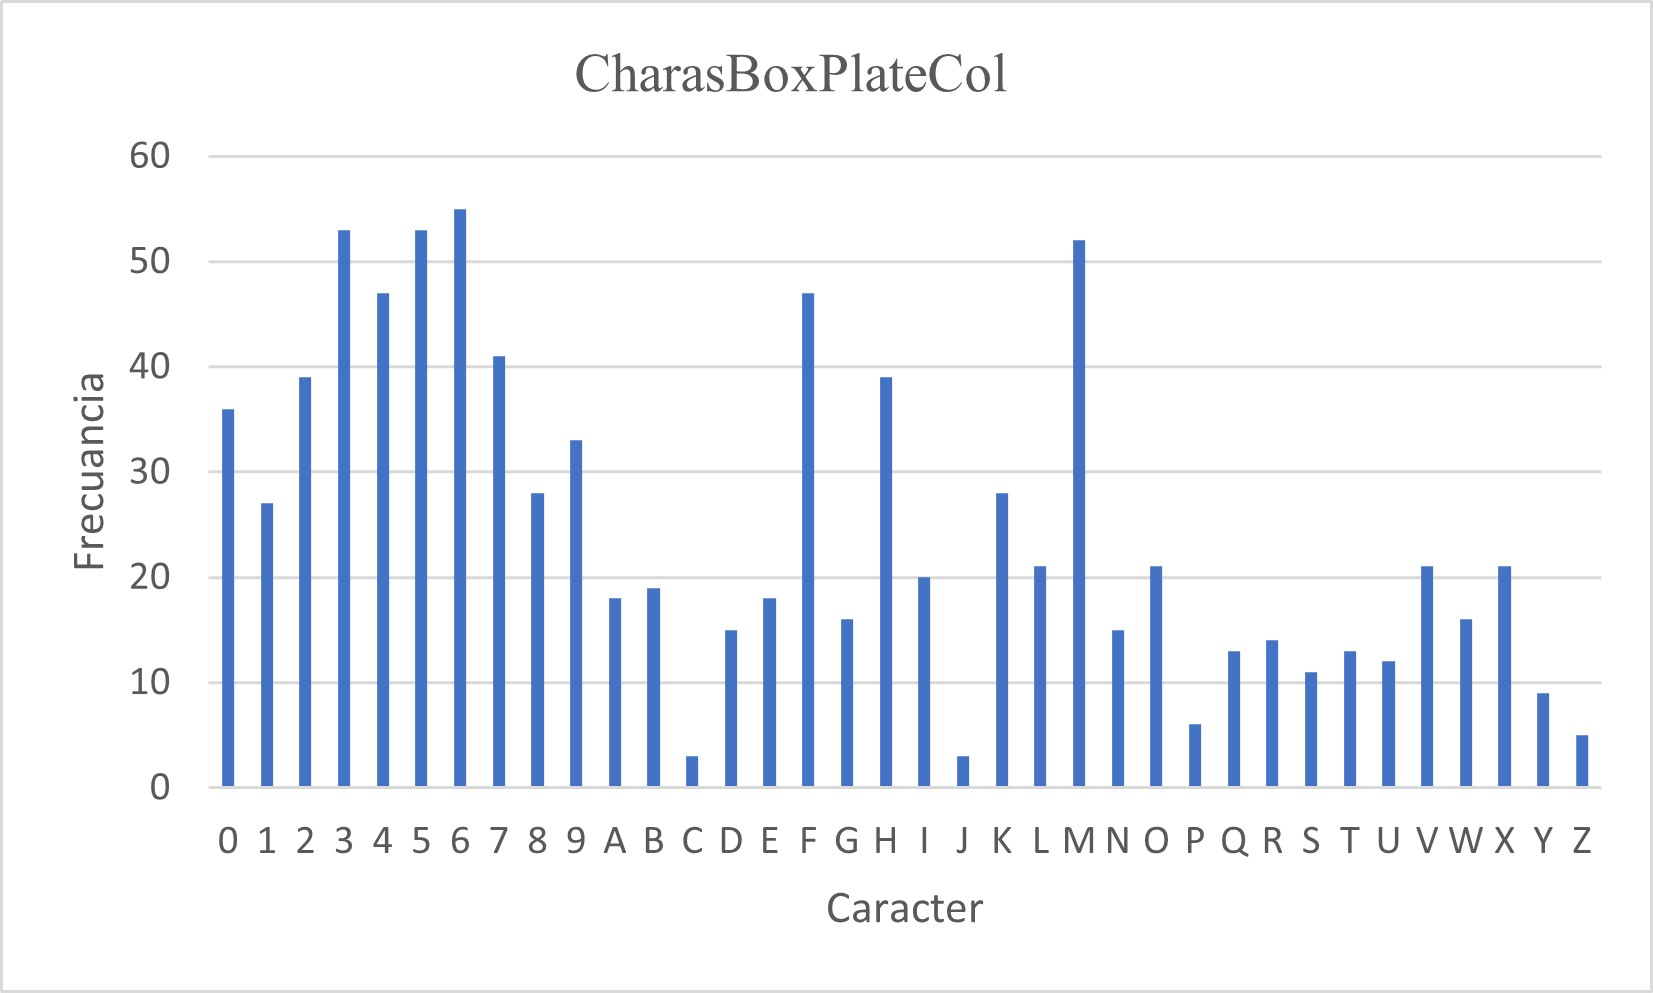
\includegraphics[width=0.8\linewidth]{imagenes/frecuenciaCaracter3.jpg}}
   \caption{Frecuencia de cada caracter en la base de datos \textit{CharsBoxPlateCol}}.
    \label{fig:frecuencia3}
\end{figure}

 \begin{tcolorbox}
[colback=green!5!white,colframe=green!45!black,fonttitle=\bfseries,title=Contribución]

   Una contribución del presente trabajo son las bases de datos \textit{CharsPlateCol} y \textit{CharsBoxPlateCol} con caracteres segmentados y etiquetados respectivamente de placas colombianas, las cuales están disponibles para cualquier investigador que las requiera para usos académicos.
\end{tcolorbox}\\

%Para tener una base de datos etiquetada con caracteres con una mayor frecuencia, se realizó una aumento de datos utilizando la aplicación RoboFlow. Ésta aplicación permite realizar muchas transformaciones de la imagen. Nosotros hemos realizado solamente cambios en el brillo (Brightness), en la rotación (Rotation), en el nivel de ruido (Noise) y en el difuminado (Blur). Estos cambios se han realizado teniendo en cuenta que se asemejan a los cambios que se pueden producir en la imagen de la placa por condiciones ambientales y por las diferentes perspectivas en que la cámara puede capturar la imagen de la placa.    
%En la tabla \ref{table:frecuencia4} se muestra la cantidad de imágenes en cada clase después de realizado el aumento de datos; y en la figura \ref{fig:frecuencia4} un diagrama de frecuencias. Se puede observar en el diagrama que se obtiene aun una base de datos muy desbalanceada, pero con mayor frecuencia en algunos caracteres.

\begin{comment}

\begin{table}[H]
\begin{center}
\resizebox{0.5\textwidth}{!}{
\begin{tabular}{||c|c||c|c||}
\hline \hline
 Clase & Frecuencia & Clase & Frecuencia\\
\hline\hline
000  &  476 & letra I  & 228 \\\hline
001  &  399 & letra J  &  83\\\hline
002  &  544 & letra K & 371\\\hline
003  & 762 & letra L & 289\\\hline
004 &  648 & letra M  & 729\\\hline
005 & 762 & letra N  &  223\\\hline
006 & 755 & letra O  & 260\\\hline
007  &  609 & letra P  &  69\\\hline
008 & 379 & letra Q & 125\\ \hline
009 & 432 & letra R & 151\\\hline
letra A  &  234 & letra S  &  119\\\hline
letra B  &  194 & letra T  &  153\\\hline
letra C  &  41 & letra U & 152\\\hline
letra D  & 211 & letra V  & 239 \\\hline
letra E  &  205 & letra W  & 186 \\\hline
letra F & 533 & letra X & 207 \\\hline
letra G  & 195 & letra Y  & 105\\\hline
letra H & 433 & letra Z  & 72\\
\hline \hline
Total etiquetas & \multicolumn{3}{|c|}{11573} \\
\hline \hline
\end{tabular}
}
\caption{\label{table:frecuencia4}Cantidad de etiquetas por clase en la base de datos \textit{CharsBoxPlateCol} con data aumentada}
\end{center}
\end{table}

\begin{figure}[H]
\centering
  {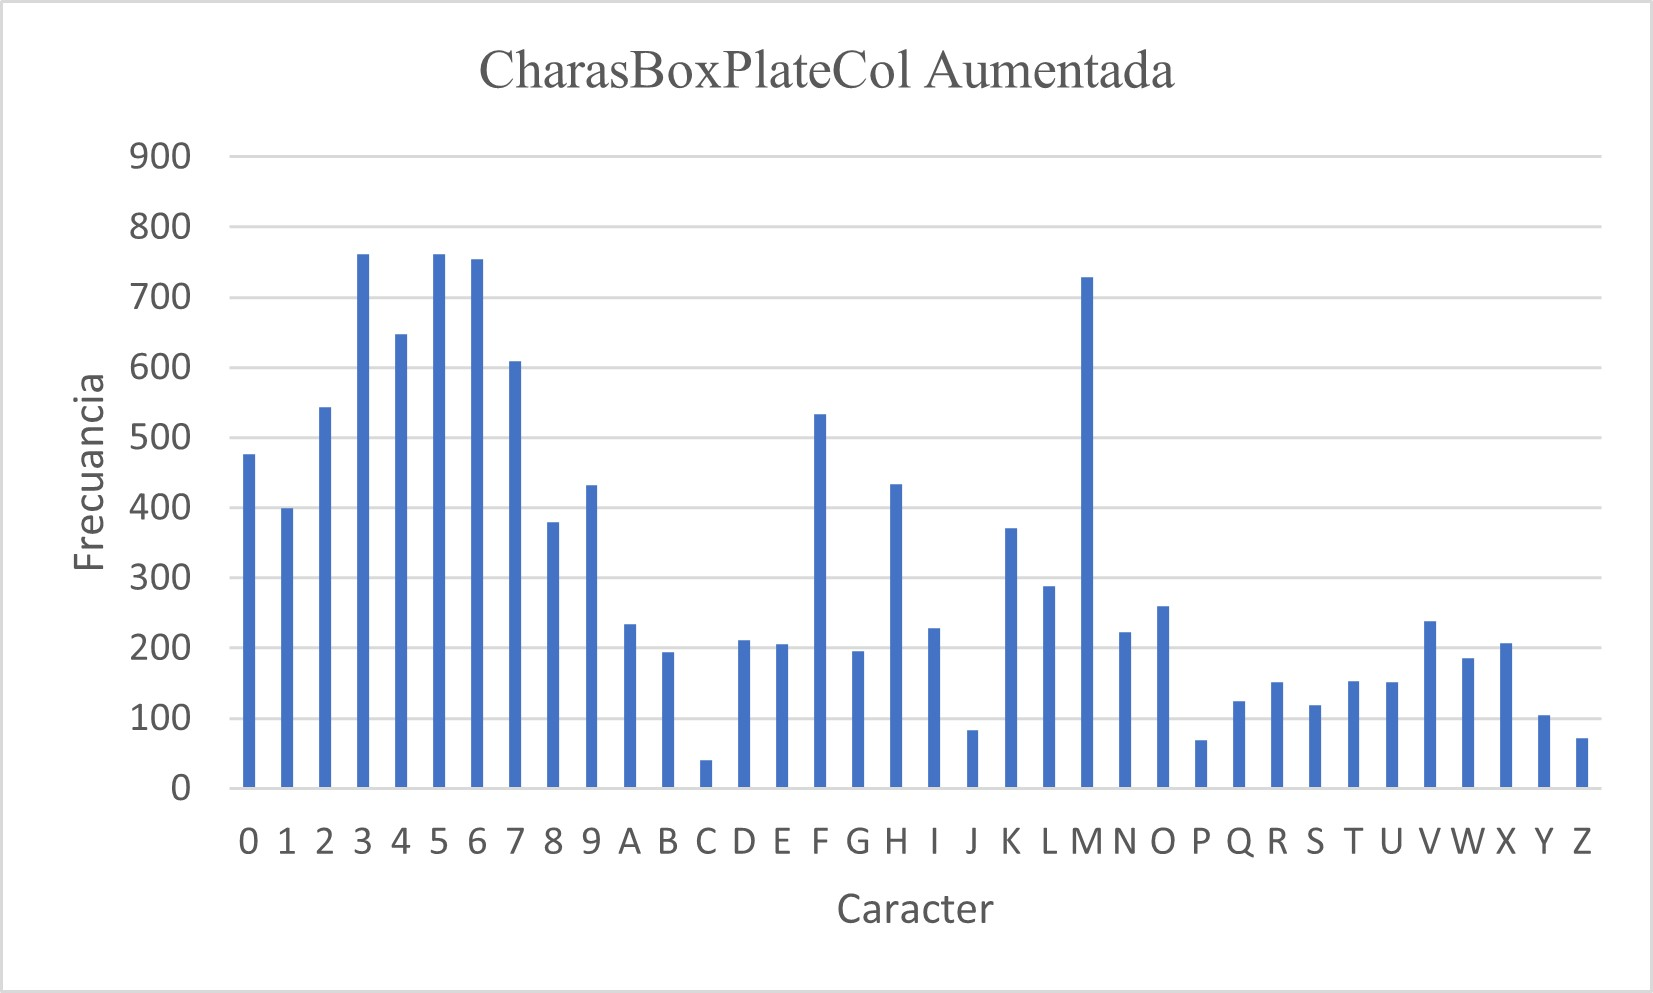
\includegraphics[width=0.7\linewidth]{imagenes/frecuenciaCaracter4.jpg}}
   \caption{Frecuencia de cada caracter en la base de datos \textit{CharsBoxPlateCol} aumentada}.
    \label{fig:frecuencia4}
\end{figure}

\end{comment}





%-----------------------------------
%La base de datos para el entrenamiento de la técnica de detección de objetos, se construye a partir de la creación de etiquetas dentro de las imágenes. Se crean cuadros delimitadores (bounding box) para cada una de las clases que se quieren detectar, independiente de la cantidad de objetos o caracteres en una misma imagen, como es nuestro caso. Por tal razón, hemos etiquetado 6 caracteres en cada una de las imágenes de la placas colombianas seleccionadas para el entrenamiento y test de nuestro modelo Faster R-CNN de tensorflow pre-entrenado.


%Se implementó una detección de objetos de tensorflow con python para el reconocimiento de caracteres en imágenes de placas vehiculares, acá es un proceso un poco diferente a la red neuronal convolucional de clasificación, ya que, en primer lugar, se detectan los 6 caracteres dentro de la misma placa que ha sido segmentada con anterioridad, lo segundo, es que hacemos una etiqueta en las imágenes que contienen la placa para el entrenamiento de la red neuronal convolucional y la construcción de la base de datos.

%Esta etapa es un pre-procesamiento de imágenes para el entrenamiento de la red neuronal convolucional mucho mas rápida con propuesta de regiones. El etiquetado se hace manualmente en los 6 caracteres en cada una de las im\'agenes predeterminadas para el entrenamiento y test, creando as'i las 36 clases que representa cada uno de los caracteres usados en las placas colombianas, esas etiquetas son cuadros delimitadores de colores por cada clase asignada.
%La etiqueta de cada uno de los caracteres dentro de la imagen de la placa se realizó con la aplicación \textbf{labelImg}, en este caso se etiquetaron 112 placas para el entrenamiento, con un promedio de 6 caracteres etiquetados por imagen, da un total de 672 etiquetas , 65 imágenes para la validación, con un promedio de 6 caracteres etiquetados para un total de 390 etiquetas\\


%\begin{figure}[H]
%\centering
%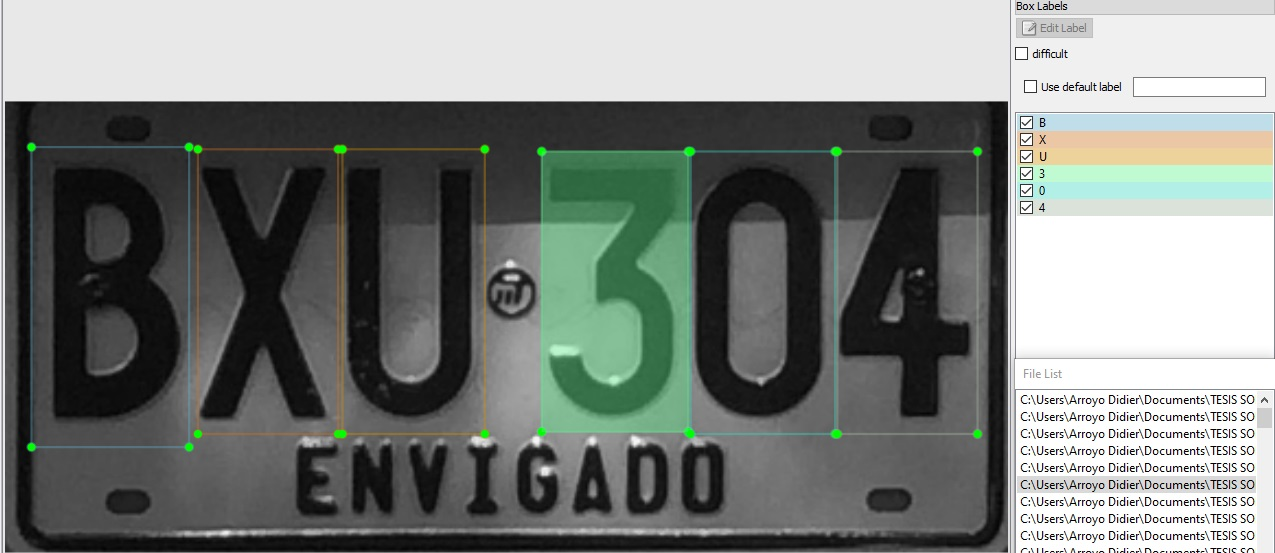
\includegraphics[width=0.5\textwidth]{imagenes/MODELO_5/ETIQUETA_MOD_IV.jpg} \caption{Caracteres etiquetados}
%\label{fig:etiquetas deteccion}
%\end{figure}

%La figura \ref{fig:etiquetas deteccion} es una muestra de las 177 placas que lograron etiquetarse, se crea un bounding box en cada clase identificada dentro de la imagen,con un color específico, este proceso genere automáticamente el documento \textbf{Xml} con las coordenadas de cada una de las clases delimitada con los cuadros.
%Este proceso se tiene que hacer manualmente con cada una de las imágenes predeterminadas para el entrenamiento de la red neuronal, donde se generará un documento \textbf{xml} por cada imagen donde se encuentran al menos unas coordenadas de las etiquetas realizadas. 

%\begin{figure}[H]
%\centering
%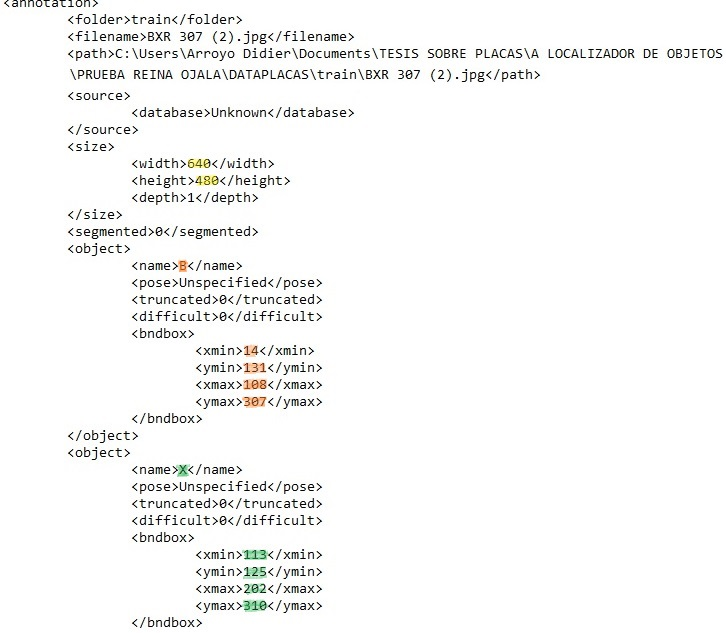
\includegraphics[width=0.7\linewidth]{imagenes/RESULTADOS/annonations.jpg} \caption{Ejemplo anotación Xml}
%\label{fig:Ejemplo anotación Xml}
%\end{figure}

%La figura \ref{fig:Ejemplo anotación Xml} es un ejemplo de la anotación de las coordenadas de las etiquetas realizadas en la imagen para la creación de la data,  en este caso podemos observar las coordenadas para las clases \textbf{B} y \textbf{X}, que gráficamente podemos observar en la figura \ref{fig:etiquetas deteccion} 

%------------------------------------------
\section{Técnicas estadísticas para el procesamiento de la información}
%---------------------------------------------------------

%La figura 5.1 muestra que la entrada del sistema son imágenes completas que incluyen vehículo y todo su contexto. Las imágenes de  entrada pertenecen a una base de datos de un parqueadero y tienen una resolución fija de 1920 x 1080. Una vez introducida una imagen, el sistema ejecutará el proceso de segmentación de la placa y luego lo hará con los caracteres que esta contiene, debemos tener en cuenta el formato de matrículas en Colombia es: tres letras y tres números. El código que realiza este primer proceso, que es la segmentación basada en la detección de contornos, se lleva a cabo con las funciones de la librería de visión artificial OpenCV.\\

En este trabajo se han usado Redes Neuronales Convolucionales para el procesamiento de la información. Consideramos que estas redes son adecuadas para superar los retos que se han planteado  en el reconocimiento de placas colombianas de automóviles, ya que presenta la ventaja de que la extracción de características viene incorporado dentro del proceso de entrenamiento de la red (ver secciones \ref{sec:antecedentes} y \ref{sec:RNC}). Nosotros hemos desarrollado dos modelos: Un primer modelo es una RNC construida desde cero e inicialmente fue entrenada utilizando solamente la base de datos \textit{CharsPlateCol} y luego fue entrenada agregándole la base de datos \textit{Chars34k}. Un segundo modelo usa la técnica de detección de objetos. Para ello hemos realizado transferencia de aprendizaje a partir de una Faster R-CNN pre-entrenada con la base de datos COCO (ver sección \ref{sec:coco}). Para entrenar la red inicialmente se usó la base de datos \textit{CharsBoxPlateCol} y después, la misma base de datos aumentada con aplicación Web RoboFlow (ver sección \ref{sec:basedatos3}).  A continuación se describen los dos modelos usados.    
%-----------------------------------------
%y  Hemos empleado en este trabajo dos técnicas para procesar la información, la primera es una Red Neuronal Convolucional 
%(RCN) la cual ser\'a la encargada del reconocimiento de caracteres en nuestro sistema después del proceso de segmentación de caracteres, igual al realizado en la creación de la data \textit{CharsPlateCol2.5k}. (ver sección \ref{CharsPlateCol2.5k}).\\ 
%La etapa de reconocimiento de caracteres realizada mediante la  red neuronal convolucional (RNC), tiene una primera fase, entrenamiento, validación y test realizado con la base de datos \textit{CharsPlateCol2.5k}, (ver sección \ref{CharsPlateCol2.5k}) para la creación de nuestro modelo 1, de igual forma entrenamos esta misma red neuronal con la base de datos \textit{Chars34k},   (Ver sección \ref{Chars34k}) para la creación de nuestro modelo 2. 
%La segunda t\'ecnica usada es la detección de objetos, se us\'o el modelo pre-entrenado de tensorflow \textbf{faster r-cnn inception v2 coco 2018 01 28} para entrenar nuestro propio clasificador de detección de objetos con una red neuronal convolucional para múltiples objetos y así poder identificar con cuadros delimitadores los caracteres en las placas colombianas, esto se hizo a partir de la técnica conocida como fine-tuning (ajuste fino).(Ver sección \ref())


%El objetivo de esta etapa es detectar aquellas regiones de la imagen que contienen los números y letras que posteriormente tratará de identificar el clasificador de la red neuronal.

%La etapa final del ejemplo de segmentación es cuando obtenemos los 6 caracteres que se extraen de toda la placa segmentada, teniendo en cuenta las dimensiones fijas de las placas colombianas. Los caracteres segmentados sirven como entrada a la red neuronal convolucional previamente entrenada, para su reconocimiento respectivo.


\subsection{Modelo 1: RNC desde cero}\label{sec:modelo1}
Este primer modelo construido desde cero consta de 3 capas de convolución seguidas de una función de activación ReLu y una capa MaxPooling. Además, una Capa de activación SoftMax con 36 salidas (26 letras y 10 números), que indican los porcentajes de clasificación obtenidos para cada clase. La tabla \ref{tab:Distribución de capas RCN} muestra su distribución de capas y parámetros.

\begin{table}[H]
    \centering
    \begin{tabular}{||c|c||}
      \hline \hline
      \textbf{Tipo de Capa} & \textbf{Cantidad}\\
      \hline \hline
      Convolucional & 5 \\
      \hline
      Densas & 3 \\
      \hline
      MaxPooling & 3 \\
      \hline
      Dropout & 2\\
      \hline
      Flatten & 1 \\
      \hline
      Total de capas & 14  \\
      \hline
      \hline
    \end{tabular}
    \caption{Distribución de capas Modelo}
    \label{tab:Distribución de capas RCN}
\end{table}

El proceso de entrenamiento de la red se basa en una estructura que relaciona unas capas convolucionales, unas capas pooling y por último una capas totalmente conectadas que nos indicará la clasificación realizada por medio de la función SoftMax.

El proceso de entrenamiento inicia con la declaración de la estructura de la red. El siguiente paso es importar el conjunto de imágenes de la base de datos. Antes de iniciar el entrenamiento, este conjunto de imágenes se divide aleatoriamente en tres subconjuntos denominados entrenamiento, validación y prueba. El conjunto de entrenamiento se utiliza para determinar los pesos de la red que permiten clasificar con el menor error posible las imágenes; el de validación para comprobar si se produce sobreajuste (\textit{overfitting}) durante el entrenamiento; y el conjunto de prueba para calcular la precisión del modelo a la hora de clasificar imágenes que no han sido utilizadas durante las épocas de entrenamiento.

El entrenamiento de esta RNC se realizó en Colaboratory \cite {Bisong2019}, un entorno gratuito de Jupyter Notebook que se ejecuta completamente en la nube.

\begin{table}[H]
\begin{center}
\begin{tabular}{||c|c|c|c||}
\hline \hline
&\textbf{Tipo de capa} & \textbf{Salida} & \textbf{No. Parámetros}\\
\hline \hline
\multirow{7}{*}{\rotatebox{90}{Ext. Características}}&\verb"conv_1(conv2D)"&(74,34,64) & 9472\\\cline{2-4}

&\verb"Activacion_1(Activacion)"& (74,34,64) & 0 \\\cline{2-4}

&\verb"pooling_1(MaxPooling2D)"&(37,17,64) &0\\\cline{2-4}

&\verb"conv_2(conv2D)"&(35,15,128) & 73856\\\cline{2-4}

&\verb"Activacion_2(Activacion)"& (35,15,128) & 0 \\\cline{2-4}

&\verb"pooling_2(MaxPooling2D)"&(17,7,128) & 0\\\cline{2-4}

&\verb"conv_3(conv2D)"&(15,5,256) & 295168\\\cline{2-4}

&\verb"Activacion_3(Activacion)""&(15,5,256) & 0 \\\cline{2-4}

&\verb"pooling_3(MaxPooling2D)"&(7,2,256) & 0\\\hline


\multirow{6}{*}{\rotatebox{90}{Clasificador}}&\verb"flatten_1(Flatten)"&(6144) & 0\\\cline{2-4}

& Dense\_1 (dense) & (1024) & 3671040 \\ \cline{2-4}
& Dropout\_1 (dropout) & (1024) & 0 \\ \cline{2-4}
& activation\_4 (activation)  & (1024) & 0 \\ \cline{2-4}
& Dropout\_2 (dropout) & (1024) & 0\\ \cline{2-4}
& Dense\_2 (dense) & (36) & 36900 \\ \cline{2-4}
& activation\_5 (Softmax) & (36) & 0\\ \hline \hline
\multicolumn{3}{||c|}{\verb"Total parámetros"}& \verb"4086436"\\
\hline
\multicolumn{3}{||c|}{\verb"Parámetros entrenables"}&\verb"4086436"\\
\hline
\multicolumn{3}{||c|}{\verb"Parámetros no entrenables"}&\verb"0"\\
\hline \hline
\end{tabular}
\caption{Estructura de la red neuronal convolucional diseñada}
\label{tab:modelo1}
\end{center}
\end{table}


\subsubsection*{Arquitectura}

Para lograr obtener una arquitectura con buen rendimiento, se realizaron varios ensayos. Inicialmente se entrenó en 50 épocas, luego se logró cambiar el entorno de entrenamiento y todos se llevaron a cabo en 200 épocas. Inicialmente el tamaño de las imágenes de entrada fueron de 32x32; luego pasaron a 50x50 y finalmente las imágenes de 80x40 píxeles con 3 canales RGB fueron las que dieron mejor resultado. Los entrenamientos se hicieron inicialmente en el entorno Jupyter en Anaconda, pero debido a la complejidad y duración excesiva de los entrenamientos (hasta 3 días), usamos el mismo entorno pero en Google Colab con acceso a trabajos con GPU totalmente gratis y en la nube. Fue así que se redujo significativamente los tiempos de entrenamiento a máximo 30 minutos. Este modelo fue entrenado con distribución de las capas descritas en el cuadro \ref{tab:Distribución de capas RCN}. La estructura de red que mejor rendimiento mostró se muestra en la tabla \ref{tab:modelo1}.

De acuerdo a la estructura de la red mostrada en la anterior tabla, cuando se tiene una imagen de entrada de 80x40 píxeles se aplica una convolución cuyo filtro es 7x7 para generar 64 mapas de características de 74x34. Un filtro de agrupación 2x2 MaxPooling se aplica a estos mapas y se obtienen 64 mapas de características de 37x17. De la misma forma lo hacemos con las siguientes convoluciones cuyos filtros son 3x3, para obtener 128 mapas de 35x15. Después de aplicar el filtro de agrupación 2x2 MaxPooling, obtenemos 128 mapas de 17x7. En la última convolución obtenemos 256 mapas de características de 15x5, que después de aplicar el filtro MaxPooling de 2x2 quedan de 7x2. Después de la etapa de extracción de características para el aprendizaje de la red, se realiza la etapa de clasificación con capas completamente conectadas. Finaliza con la función de activación Softmax, que asigna probabilidades de reconocimiento a cada una de las clases para finalmente realizar la clasificación de los caracteres en la placa de entrada.

\begin{table}[H]
\begin{center}
\begin{tabular}{||c|c||c|c||}
\hline
\hline
 Índice & clase & Índice & clase  \\
\hline
0 & letra P & 18 & letra Q\\ \hline
1 & 001 & 19 & 004\\ \hline
2 & letra O & 20 & letra U\\ \hline
3 & 008  & 21 & letra A\\ \hline
4 & letra D & 22 & 005\\ \hline
5 & letra M & 23 & letra Y\\ \hline
6 & letra N & 24 & letra L\\ \hline
7 & letra B & 25 & letra R\\ \hline
8 & 002 & 26 & letra G\\ \hline
9 & 003 & 27 & letra Z\\ \hline
10 & letra I & 28 & letra K\\ \hline
11 & letra E & 29 & letra J\\ \hline
12 & 007 & 30 & 009\\ \hline
13 & letra S & 31 & 000\\ \hline
14 & letra F & 32 & letra X\\ \hline
15 & 006 & 33 & letra V\\ \hline
16 & letra C & 34 & letra H\\ \hline
17 & letra W & 35 & letra T\\ \hline \hline

\hline
\end{tabular}
\caption{\label{table:indices_data segmentada}índices asignados a cada una de las 36 clases a clasificar}
\end{center}
\end{table}


\subsection{Entrenamiento}\label{sec:entreModelo1}

La tabla \ref{table:indices_data segmentada} muestra los índices asignados a cada una de las 36 clases a clasificar (caracteres de placas colombianas).


La tabla \ref{table:Datos de entrenamiento} muestra los parámetros utilizados para el entrenamiento del modelo 1, los cuales fueron los que dieron mejor rendimiento después de múltiples ensayos.

\begin{table}[H]
\begin{center}
\begin{tabular}{||c|c||}
\hline
 Parámetros &  \\
\hline
\hline
longitud-altura imagen & 80 x 40\\ \hline
Imágenes de entrenamiento & 1659 \\ \hline
Imágenes de validación & 415\\\hline
Imágenes de test & 519\\\hline
INIT LR & 0.001 \\\hline
épocas & 200 \\\hline
batch size & 16\\ \hline
optimizador & SGD\\\hline
\hline
\hline
\end{tabular}
\caption{\label{table:Datos de entrenamiento} Parámetros usados en el entrenamiento del Modelo 1}
\end{center}
\end{table}



\subsection{Modelo 2: Faster R-CNN pre-entrenado}

Este modelo fue construido a partir del modelo  pre-entrenado de detección de objetos \textbf{Faster R-CNN Inception v2 (COCO)} de TensorFlow.

Se realizó transferencia de aprendizaje para entrenar nuestro propio clasificador de detección de objetos, en nuestro caso, caracteres en la imagen de una placa.  La identificación se realiza con cuadros delimitadores en cada uno de los caracteres en las placas colombianas. Esto se hizo a partir de la técnica conocida como fine-tuning (ajuste fino), que consiste en realizar un ajuste de la red inicializando con los pesos ya obtenidos del modelo pre-entrenado (inferencia). En la tabla \ref{tab:Distribución de redes} se encuentra la distribución de redes y capas que conforman una \textbf{Faster R-CNN}. Está cosntituida por tres redes (RNC, RPN y R-CNN) y una capa RoIP (ver sección \ref{sec:Faster}). 

\begin{table}[H]
    \centering
    \begin{tabular}{||c|c||}
      \hline \hline
      \textbf{Tipo de red o capa} & \textbf{Cantidad}\\
      \hline \hline
      RNC & 1 \\
      \hline
      Red de propuesta de región (RPN) & 1 \\
      \hline
      Capa de agrupación de regiones de interés (RoIP)  & 1 \\
      \hline
      R-CNN & 1\\
      \hline
      Total & 4  \\
      \hline
      \hline
    \end{tabular}
    \caption{Distribución de redes y capas Modelo}
    \label{tab:Distribución de redes}
\end{table}

%Dividimos nuestra data en dos directorios train y test. El modelo solo usará imágenes del directorio "train" para entrenamiento e imágenes de la carpeta "test" para evaluar el rendimiento del modelo, luego cargamos imágenes nunca antes vista por el modelo para la prueba.
%Debemos generar dos archivos train.record y test.record, ambos son archivos binarios, cada uno contiene el jpg codificado y la información de anotación del cuadro delimitador para el conjunto de train y test correspondiente. El formato de archivo tfrecord es más fácil de usar y más rápido de cargar durante la fase de entrenamiento en comparación con el almacenamiento de cada imagen y anotación por separado. Este archivo tfrecord se genera a partir del documento \textbf{XML} que contiene las anotaciones de la etiquetas, esta información genera dos archivos, uno de los label y otro con las anotaciones de las etiquetas que finamente genere el archivo tfrecord para train y test. 